\documentclass[aoas,preprint]{imsart}

\RequirePackage[OT1]{fontenc}
\RequirePackage{amsthm,amsmath}
\RequirePackage{natbib}
%\RequirePackage[nameyear]{natbib}
\RequirePackage[colorlinks,citecolor=blue,urlcolor=blue]{hyperref}

\usepackage{amssymb, amsmath}
\usepackage{algorithm}
\usepackage{algorithmic}
\usepackage{xfrac}

\DeclareMathOperator*{\argmin}{arg\,min}
\DeclareMathOperator*{\argmax}{arg\,max}
\newcommand{\citek}[1]{[\cite{#1}]}

% settings
%\pubyear{2005}
%\volume{0}
%\issue{0}
%\firstpage{1}
%\lastpage{8}
\arxiv{arXiv:0000.0000}

\startlocaldefs
\numberwithin{equation}{section}
\theoremstyle{plain}
\newtheorem{thm}{Theorem}[section]
\endlocaldefs

\begin{document}

\begin{frontmatter}
%\title{Approximating Generalized Likelihood Ratio Tests with Calibrated Discriminative Classifiers}
%\title{Approximating  Likelihood Ratio Tests with Calibrated Discriminative Classifiers}
\title{Approximating  Likelihood Ratios with Calibrated Discriminative Classifiers}
%\title{Approximating Likelihood Ratio Tests with Calibrated Classifiers}
%\title{A Sample Document\thanksref{T1}}
\runtitle{Approximating Likelihood Ratios with Classifiers}
%\thankstext{T1}{Footnote to the title with the ``thankstext'' command.}

\begin{aug}
\author{\fnms{Kyle} \snm{ Cranmer}\thanksref{t1}\ead[label=e1]{kyle.cranmer@nyu.edu}}
%,
%\author{\fnms{Second} \snm{Author}\thanksref{t3,m1,m2}\ead[label=e2]{second@somewhere.com}}
%\and
%\author{\fnms{Third} \snm{Author}\thanksref{t1,m2}
%\ead[label=e3]{third@somewhere.com}
%\ead[label=u1,url]{http://www.foo.com}}

\thankstext{t1}{US National Science Foundation grants PHY-0854724 and PHY-0955626.}
%\thankstext{t2}{First supporter of the project}
%\thankstext{t3}{Second supporter of the project}
\runauthor{K. Cranmer}

\affiliation{Center for Cosmology \and Particle Physics\thanksmark{m1} \\
       \and Center for Data Science\thanksmark{m2}
       New York University}

\address{Center for Cosmology and Particle Physics\\
       New York University \\
       New York, NY 10003, USA
\phantom{E-mail:\ }\printead*{e1}}
\end{aug}


\begin{abstract}%   <- trailing '%' for backward compatibility of .sty file
In particle physics likelihood ratio tests are established tools for statistical inference. 
These tests are complicated by the fact that computer simulators are used as a generative model for 
the data, but they do not provide a way to evaluate the likelihood function. 
We demonstrate how discriminative classifiers can be used to approximate the likelihood function when 
a generative model for the data is available for training and calibration.  This offers an approach to parametric inference when simulators are used that is complementary to approximate Bayesian computation.
\end{abstract}

\begin{keyword}[class=MSC]
\kwd[Primary ]{62P35}
\kwd{62F99}
\kwd[; secondary ]{62H30}
\end{keyword}

\begin{keyword}
\kwd{likelihood ratio}
\kwd{classification}
\kwd{particle physics}
\end{keyword}

\end{frontmatter}

\section{Introduction}
%\subsection{}

The likelihood function is the central object that summarizes the information from an experiment needed for inference of model parameters. The likelihood function is key to Bayesian inference, and many areas of science that report the results of classical hypothesis tests or confidence intervals use the (generalized or profile) likelihood ratio as a test statistic.
%  are established tools for statistical inference~\citek{Wilks1938}. 
It is increasingly common that a simulator (or generative model) is used to describe complex processes that tie 
parameters $\theta$ of an underlying theory and measurement apparatus to high-dimensional observations $x$. 
Directly evaluating the likelihood ratio in these cases is often impossible or is computationally impractical. 
Approximate Bayesian Computation (ABC) is one approach to parameter inference in this simulation-based or likelihood-free setting~\citek{Rubin1984,Tavare1997,Marin2011}. Here we consider an alternative approach that can also be used in a classical setting where a prior over the parameters is not available. In particular, we demonstrate how discriminative classifiers can be used to construct equivalent likelihood ratio tests when a generative model for the data is available for training and calibration.  

As a concrete example, consider searches for new particles at the Large Hadron Collider. 
The simulator that is sampling from $p(x|\theta)$ is based on quantum field theory, a detailed simulation of the particle detector, and data processing algorithms that transform raw sensor data into the feature vector $x$~\citek{Sjostrand:2006za,Agostinelli:2002hh}.  


The ATLAS and CMS experiments have published  hundreds papers where the 
final  result was formulated as a hypothesis test or confidence interval 
using a generalized  likelihood ratio test~\citek{Cowan:2010js}. This includes
the discovery of the Higgs boson~\citek{Aad:2012tfa,Chatrchyan:2012ufa} and 
subsequent measurement of its properties.  

The bulk of the likelihood ratio tests at the LHC are based on the distribution of a single event-level feature
that discriminates between a hypothesized process of interest (labeled \textit{signal}) and various other processes 
(labeled \textit{background}). Typically,  pseudo-data from the simulator are used to approximate the density
at various parameter points, and an interpolation algorithm is used to approximate the parametrized model~\citek{Cranmer:2012sba}.


To improve the statistical power of these tests, hundreds of these searches have utilized supervised learning to train discriminative classifiers that take advantage of a high dimensional feature vector $x$. Within High Energy Physics (HEP) libraries such as TMVA that implement conventional techniques like the multi-layer perceptron and boosted decision trees~\citek{Hocker:2007ht} are commonly used. Recently, there has been progress in using deep networks~\citek{Baldi:2014kfa} and a NIPS workshop synthesizing the lessons learned during HiggsML~\citek{HepML}, the largest Kaggle challenge in history. 
%The use of classifiers is effective, but an intermediate step not obviously connected to the target likelihood ratio test.

%Collisions are usually selected with supervised learning methods 
While classification accuracy can lead to optimal approaches for simple hypothesis tests~\citek{Dempster1965}, that is no longer true in the context of parameter estimation or composite hypothesis tests with nuisance parameters. As noted in ~\citek{Whiteson:2006ws}, ``such methods are suboptimal because they assume that the selector with the highest classification accuracy will yield a mass measurement with the smallest statistical uncertainty.''
%In what follows, it will be important to distinguish between the per-event loss used for classification, and the per-experiment loss 
The key distinction is that evaluating the loss for classification is composed of many per-event operations, while evaluating the loss for a mass measurement (e.g. the variance of an estimator for the mass parameter) is a per-experiment operation involving a data set with many events. They went on to demonstrate a computationally intensive stochastic optimization technique based on the per-experiment loss out performed the two stage selection-estimation process. 
%This paper shows that (to the extent a generalized likelihood ratio test in the full feature space is close to  optimal) one can achieve optimal results with a  specific per-event procedure by reformulating the target likelihood ratio in terms of a per-event classification followed by an specific calibration process.

The initial motivation for this work was to extend the typical usage of discriminative classifiers in HEP to be robust to 
nuisance parameters in the simulators. The scope of the result expanded once it became clear that this offers a way to approximate the likelihood function $p(x|\theta)$ in what is typically considered the likelihood-free setting. This approach is complementary to ABC as it does not require a prior over the parameters and can also be used in the classical (frequentist) setting.  In Section~\ref{S:Related} we discuss the scheme sketched by \cite{Neal:2007zz} that also suggests using a classifier  as a dimensionality reduction map to aid in the estimation of the likelihood function.


%In the context of machine learning or decision theory one starts with a well defined loss function.
%In order to define a Bayes risk one must also specify a prior over the parameters.
%%In practice, it can be difficult, particularly for large collaborations, to agree on such high-level topics.
%In practice, large particle physics collaborations have preferred to avoid specifying the 
%high-level loss function and prior, and instead accepted the properties of generalized likelihood ratio tests.
%Thus, we will not try to specify a loss function other than to approximate the generalized likelihood ratio itself.
%
%The form of the generalized likelihood ratio is explicitly a per-experiment object, thus naively it has the same computational challenges as other approaches that optimize a per-experiment loss. 
%This paper shows how one can reformulate generalized likelihood ratio test in terms of a per-event classification stage and a calibration process. Moreover, one can utilize a generative statistical model for the data both to train a discriminative classifier with a supervised learning algorithm and for the calibration process.
%In Section~\ref{S:Related} we discuss the scheme sketched by \cite{Neal:2007zz} that also suggests using a classifier  as a dimensionality reduction map to aid in the estimation of the likelihood function.


%\bigskip
%
%Generalized likelihood ratio tests enjoy a number of optimal properties in the asymptotic limit and are widely used even away from that limit. These asymptotic properties, the difficulty in specifying a prior over the parameters needed to evaluate a Bayes risk, and the vast literature associated to likelihood ratio tests has led many users of such tests to not be explicit about the loss function they wish to minimize for their experiment. Thus, we will not try to specify a loss function other than to approximate the generalized likelihood ratio itself. The form of the generalized likelihood ratio is explicitly a per-experiment object, thus naively it has the same computational challenges as other approaches that optimize a per-experiment loss. 

%Similarly,~\cite{Neal:2007zz} suggested using a classifier as a dimensionality reduction map to aid in the estimation of the likelihood function. We discuss the key differences with that work in Section~\ref{S:Related}.

%This paper shows how one can reformulate generalized likelihood ratio test in terms of a per-event classification stage and a calibration process. Moreover, one can utilize a generative statistical model for the data both to train a discriminative classifier with a supervised learning algorithm and for the calibration process.


%This paper describes how one can utilize generative statistical models for the data in conjunction with discriminative classifiers to construct generalized likelihood ratio tests that are equivalent to 
%the one that would have been obtained if it were possible to evaluate the probability 
%density implicitly being sampled by the generative model.
%
%This paper describes how one can utilize generative statistical models for the data in conjunction with discriminative classifiers to construct generalized likelihood ratio tests that are equivalent to 
%the one that would have been obtained if it were possible to evaluate the probability 
%density implicitly being sampled by the generative model.

%The labeled data used to train the classifiers are not obtained from the experimental apparatus. 
%Instead they are generated from a 
%detailed simulation, which includes a quantum mechanical description of the underlying particle 
%interactions, an exquisitely detailed simulation of the particle detectors with hundreds of millions of 
%sensors, and the data processing pipeline that reduces the data for a single event to tens or hundreds of high-level features used as input to the classifier. 
%It takes several minutes for this generative model to simulate a single collision or \textit{event} with Monte Carlo
%techniques. While particle physics offers an extreme example, it is common in science that generative 
%models are available while it not feasible to evaluate the probability density function that is implicitly being 
%sampled by the generative model.

  

\subsection{Notation and Assumptions}

We use the following notation:
\begin{itemize}
 \item $x$: a vector of features for an event
 \item $D$: a data set of $D=\{x_1, \dots, x_n\}$, where $x_e$ are assumed to be i.i.d.
 \item $\theta$: parameters of a statistical model
\item $p(x| \theta)$:  probability density  (simulation-based model) for $x$ given $\theta$
%\item $s(x)$: real-valued score from a machine learning classification algorithm (or any map $s: X\to\mathbb{R}$)
\item $y$: a class label used for training a classifier.
\item $s(x;\theta_0, \theta_1)$: real-valued discriminative classification score, parametrized by $\theta_0$ and $\theta_1$
%\item $p( s | \theta )$ The probability density function for $s$ implied by $p(x|\theta)$ and $s(x)$
\item $p( s_{\theta_0, \theta_1} | \theta )$: The probability density  for $s(x; \theta_0, \theta_1)$ implied by $p(x|\theta)$ 
\end{itemize}
We will assume the $x_e$ are i.i.d., so that $p(D|\theta) = \prod_{e=1}^n p(x_e | \theta)$.

%\newpage
\subsection{Prelude}

In the setting where one is interested in simple hypothesis testing between a null $\theta=\theta_0$ against an alternate $\theta=\theta_1$, the Neyman-Pearson lemma states that the likelihood ratio 
\begin{equation}
T(D) = \prod_{e=1}^n \frac{ p(x_e|\theta_0)}{ p(x_e|\theta_1)}
\end{equation}
is the most powerful test statistic. In order to evaluate $T(D)$, one must be able to evaluate the probability density 
$p(x| \theta)$ at any value $x$. However, it is increasingly common in science that one has a complex simulation that 
can act as generative model  for $p(x|\theta)$, but one cannot evaluate the density directly. For instance, this is the case 
high energy physics where the simulation of particle detectors can only be done in the `forward mode'. This same setting has been considered by \cite{ClaytonScott}, \cite{JMLR:v14:tong13a}, and \cite{Neal:2007zz}.

The main result of this paper is to generalize the observation that one can form an equivalent test based on 
%\begin{equation}
%T'(D) = \prod_{e=1}^n \frac{ p(\,s(x_e; \theta_1, \theta_0) \mid \theta_1)}{ p(\,s(x_e; \theta_1, \theta_0)\mid\theta_0)}
%\end{equation}
\begin{equation}\label{eq:equivLRtest}
T'(D) = \prod_{e=1}^n \frac{ p(s_e | \theta_0)}{ p(s_e | \theta_1)}
\end{equation}
if 
\begin{equation}\label{eq:montonic}
s_e = s(x_e; \theta_0, \theta_1) = m\left(\, p(x_e|\theta_0) / p(x_e|\theta_1) \,\right) \; 
%s_e = s(x_e; \theta_0, \theta_1) = m\left(\frac{ p(x_e|\theta_0)}{ p(x_e|\theta_1)} \right) \; 
\end{equation}
where $m$ is any strictly increasing or decreasing function. This result will be proven below.
This allows us to recast the original likelihood ratio test into an alternate form in which supervised learning is used to train the discriminative classifier $s(x; \theta_0, \theta_1)$. The discriminative classifier can be trained with data $(x,y=0)$ generated 
from $p(x|\theta_0)$ and $(x,y=1)$ generated from $p(x|\theta_1)$. In Section~\ref{S:GLR} we extend this result to generalized likelihood ratio tests, where it will be useful to have the classifier  parametrized in terms of $(\theta_0, \theta_1)$.

Here we see that the original goal for simple hypothesis testing (i.e. to make a decision to accept or reject the null hypothesis based on the entire data set $D$) has been reformulated into a per-event classification problem. This follows from the fact that we assume the $x_e$ to be i.i.d.

\subsection{Comments on classification and frequentist hypothesis tests}

Vast literature exists around generative and discriminative classifiers~\citek{AndrewY.Ng}. Typically, generative classifiers learn a model for the joint probability $p(x,y)$, of the inputs $x$ and the classification label $y$, and predict $p(y|x)$ via Bayes rule. In contrast, discriminative classifiers model the posterior $p(y|x)$ directly. For classification tasks, one then thresholds on $p(y|x)$. In both cases this description in terms of a posterior requires a prior distribution for $p(y)$, which is either modeled explicitly or learned from the training data. 
This familiar formulation of classification may lead to some confusion in the setting of the current work. 

The first possible source of confusion we wish to avoid is that here $p(x|\theta)$  is a  \textit{generative statistical model} for the features $x$, not a generative classifier. We think of the  $p(x|\theta)$ along the lines of a traditional scientific theory or simulator, able to make predictions about $x$ and being motivated by domain-specific considerations. 
%For example, in the context of HEP $p(x|\theta)$ is based on quantum field theory, a detailed simulation of the particle detector, and data processing algorithms that transform raw sensor data into the feature vector $x$~\citek{Sjostrand:2006za,Agostinelli:2002hh}.  
%Moreover, we are not attempting to learn the generative model $p(x|\theta)$, we are taking it as given and trying to learn the corresponding (generalized) likelihood ratio test.
%The point here is to make the distinction of $p(x|\theta)$ in this context from a generic generative classifier like normal discriminate analysis or naive Bayes. 

The second possible source of confusion is that 
we are not directly interested in calibrating the classification score in terms of a per-event posterior probability $p(y|x)$. 
Instead, we are interested in the approximation of the per-experiment likelihood function or likelihood ratio, which might be used for several purposes, including the calculation of p-values.
% defined by $P(T(D) > k |\theta)$.
%
%%the likelihood ratio $T(D)$ is aimed at tests based on the entire data set; 
%we are not interested in thresholded classification on individual events $x_e$.  
%Knowing that classifier scores are often poorly calibrated is an immediate concern.

%We wish to have well calibrated p-values defined by $P(T(D) > k |\theta)$, not well calibrated posterior probabilities $p(y|x)$. 

Lastly, in the setting of frequentist hypothesis tests and confidence intervals, we do not have a prior $\pi(\theta)$. 
While we can use the generative models to produce training data $(x,y=0)$ generated 
from $p(x|\theta_0)$ and $(x,y=1)$ generated from $p(x|\theta_1)$, the relative mix $p(y)$ 
is arbitrary.  When $p(y=0)=p(y=1)=\sfrac{1}{2}$, then 
\begin{equation}
p(y=1 | x) = \frac{p(x|y=1)}{p(x|y=0)+p(x|y=1)} = \frac{p(x|\theta_1)}{p(x|\theta_0)+p(x|\theta_1))} \;,
\end{equation}
which is monotonic with the desired likelihood ratio $p(x|\theta_1)/p(x|\theta_0)$.
Since the prior $p(y)$ is not needed for the target likelihood ratio test and because the classifier score $p(y|x)$ may not be well calibrated, we choose to denote the classifier score $s(x)$ and simply think of it as a deterministic dimensionality reduction map $s: X \to \mathbb{R}$.  Similar points have been made by~\cite{ClaytonScott} and \cite{Neal:2007zz}.


% and we need not
%interpret the balance of the training data in terms of a prior probability for the two hypotheses.
%free from the
%complications of the prior $\pi(\theta)$ that is undefined in the frequentist context.



\section{Dimensionality reduction and calibration}


We are interested in reformulating the target likelihood ratio  
\begin{equation}
\ln T =   \sum_{e=1}^n \underbrace{\log \left[ \frac {p(x_e | \theta_0) }{ p(x_e | \theta_1) } \right]}_{q(x_e)} \;.
\end{equation}
This is equivalent to approximating the likelihood function for $\theta_0$  when $\theta_1$ is held fixed.
Here we see that the test statistic $T$ for the experiment is composed of a sum over events of the per-event function $q(x)$. A sum over a monotonic, but non-linear function of $q(x)$ would not lead to an equivalent statistic. 

The important part of the per-event function $q(x)$ is that it defines iso-contours in the feature space $x$. As we will show, our goal is to learn a monotonic function of $p(x|\theta_0)/p(x|\theta_1)$, which will share the same iso-contours. Then the remaining challenge is to find the appropriate monotonic function that gives back a linear function of $q(x)$. Our claim is that the generative model $p(x|\theta)$ can be used to calibrate the density $p(s|\theta)$ and that
\begin{equation}\label{eq:envoloping}
\ln T' = \sum_{e=1}^n \underbrace{\log \left[ \frac {p(s_e | \theta_0) }{ p(s_e | \theta_1) } \right]}_{q(s_e)} \;,
\end{equation}
leads to an equivalent statistic.

For notational simplicity, let $p_0(x) = p(x|\theta_0)$, $p_1(x) = p(x|\theta_1)$, and $s(x)=s(x; \theta_1, \theta_0)$.
The distribution of $x$ totally determines the distribution of $s$. 
In the application at hand, the function $s$ maps a high-dimensional feature vector $x$ to $\mathbb{R}^+$.
Let $\Omega_{c}$ be the level set $\{x \mid s(x) = c \}$ and $\hat{n}=\nabla s(x) / |\nabla s(x)|$ be the orthonormal vector to $\Omega_c$ at the point $x$.

We need to show that for all $x$, the density
\begin{equation}
p(q_x|\theta) = \int dx \delta(q_x-q_x(x)) p(x|\theta)  / | \hat{n} \cdot \nabla q_x  | 
\end{equation}
is equal to the density
\begin{equation}
p(q_s|\theta) = \int dx \delta(q_s-q_s(s(x))) \, p(x|\theta) \, / | \hat{n} \cdot \nabla q_s  | \; .
\end{equation}
It is sufficient to show that $q_x(x) = q_s(s(x))$ $ \forall x\in\Omega_c$. The function $q_s(s)$ is based on the induced densities $p_0(s)$ and $p_1(s)$.  The induced density $p_1(c)$ is given by 
\begin{equation}
p_1(c) = \int dx \delta(c-s(x)) p_1(x) = \int d\Omega_c p_1(x)  / | \hat{n} \cdot \nabla s  |
\end{equation}
and a similar equation for $p_0(c)$. 
%\textbf{Do we need Jacobian for x $\to$ s independent of delta function part, I think that's double counting?}

\textbf{\flushleft Theorem 1:}
We have the following equality
\begin{equation}
\frac{p_1(c)}{p_0(c)} =  \frac{p_1(x)}{p_0(x)}  \;\hspace{3em} \forall x\in\Omega_c.
\end{equation}
\textbf{Proof}
For $x\in \Omega_c$, we can factor out of the integral the constant $p_1(x)/p_0(x)$.
Thus
\begin{equation}
p_1(c) = \int dx \delta(c-s(x)) p_1(x) = \int d\Omega_c p_1(x) / | \hat{n} \cdot \nabla s  |= \frac{p_1(x)}{p_0(x)} \int d\Omega_c p_0(x)  / | \hat{n} \cdot \nabla s  | \;,
\end{equation}
and the integrals cancel in the likelihood ratio
\begin{equation}
\frac{p_1(c)}{p_0(c)} = \frac{p_1(x)}{p_0(x)} \frac{\int d\Omega_c p_0(x)/ | \hat{n} \cdot \nabla s  |}{ \int d\Omega_c p_0(x) / | \hat{n} \cdot \nabla s  |} = \frac{p_1(x)}{p_0(x)}  \;\hspace{3em} \forall x\in\Omega_c.
\end{equation}

One can think of the ratio $p_1(s)/p_0(s)$ as a way of calibrating the the discriminative classifier and correcting for the monotonic transformation $m$ of the desired likelihood ratio as in Eq.~\ref{eq:montonic}.

%\bigskip
%In the case of simple hypothesis testing, $\theta_0$ and $\theta_1$ are specified and there is a unique map $s(x) =  s(x_e; \theta_0, \theta_1)$. In that case, the equivalent likelihood ratio test can be performed by first transforming the data to $D_s = \{s_1, \dots, s_e\}$, constructing the likelihoods
%\begin{equation}\label{eq:NP}
%p( D_s \,|\,  \theta) = \prod_{e=1}^n \,  p( s_e \, |\,  \theta)   \; 
%\end{equation}
%for $\theta=\{\theta_0,\theta_1\}$, and constructing the likelihood ratio based on $p(D_s|\theta_0)/p(D_s|\theta_1)$.



\section{Composite hypotheses and the generalized likelihood ratio}\label{S:GLR}

In the case of composite hypotheses $\theta \in \Theta_0$ against an alternative $\theta \in \Theta_0^C$, the generalized likelihood ratio\footnote{Also known as the profile likelihood ratio.} test is commonly used
\begin{equation}
\lambda(\Theta_0) =  \frac{ \sup_{\theta \in \Theta_0} p(D | \theta)}{ \sup_{\theta \in \Theta} p(D | \theta)} \; .
\end{equation}
This generalized likelihood ratio can be used both for hypothesis tests in the presence of nuisance parameters or to create confidence intervals with or without nuisance parameters.  Often, the parameter vector is broken into two components $\theta=(\mu,\nu)$, where the $\mu$ components are considered parameters of interest while the $\nu$ components are considered nuisance parameters. In that case $\Theta_0$ corresponds to all values of $\nu$ with $\mu$ fixed.

Denote the maximum likelihood estimator
\begin{equation}\label{eq:mle}
\hat{\theta} = \argmax_\theta  p(D | \theta)
\end{equation}
and the conditional maximum likelihood estimator
\begin{equation}\label{eq:cmle}
\hat{\hat{\theta}} = \argmax_{\theta \in \Theta_0}  p(D | \theta) \; .
\end{equation}

It is not obvious that if we are working with the distributions $p(s|\theta)$ (for some particular $s(x; \theta_0, \theta_1)$ comparison) that we can find the same estimators. 
Fortunately, there is a construction based on $p(s|\theta)$ that works. The maximum likelihood estimate of Eq.~\ref{eq:mle} is the same as the value that maximizes the likelihood ratio with respect to $p(D|\theta_1)$ for some fixed value of $\theta_1$. This allows us to use Theorem~1 to reformulate the maximum likelihood estimate
\begin{equation}\label{eq:mle_withs}
\hat{\theta} = %\argmax_\theta \frac{ p(D | \theta)}{ p(D | \theta_1)} = 
\argmax_\theta  \sum \ln \frac{p(x_e | \theta)}{p(x_e|\theta_1)} = \argmax_\theta  \sum \ln \frac{p(s(x_e; \theta, \theta_1) | \theta)}{p(s(x_e; \theta, \theta_1) |\theta_1)} \; .
\end{equation}
It is important that we include the denominator $p(s(x_e; \theta, \theta_1) |\theta_1)$ because this cancels Jacobian factors that vary with $\theta$.

\section{Learning the correct mapping and its distribution}\label{S:classifier}

Thus far we have shown that likelihood ratio tests based on $p(x|\theta_0)/p(x|\theta_1)$ with high dimensional features $x$ can be reproduced via hypothesis tests based on the univariate densities $p(s|\theta)$ for the particular dimensionality reduction map $s(x|\theta_0, \theta_1)$.
% Often it is not possible to evaluate the density $p(x|\theta)$ at a given point $x$.  
%This approach will not be useful if it is not possible to approximate $s(x|\theta_0, \theta_1)$ and $p(s|\theta)$ without evaluating the density $p(x|\theta)$. 
%In order for this approach to be useful, we need to be able to approximate both based on samples $\{(x,\theta)\}$ drawn from the generative model $p(x|\theta)$.  
In order for this approach to be useful in the likelihood-free setting where it is not possible to evaluate the density $p(x|\theta)$, we need to be able to approximate both $s(x|\theta_0, \theta_1)$ and $p(s|\theta)$ based on samples $\{x_i\}$ drawn from the generative model $p(x|\theta)$.  

Denote the approximate dimensionality reduction map $\hat{s}(x; \theta_0, \theta_1)$ and its distribution $\hat{p}(\hat{s}|\theta)$. In general we will be interested in the machine learning problem that approximates these distributions based on samples $\{x_i\}$ drawn from the generative model $p(x|\theta)$.  
The first step in this direction is to confirm that a discriminative classifier obtained from common supervised learning algorithms will yield a function that is one-to-one with $p(x|\theta_0)/p(x|\theta_1)$.
%In particular, 
%is there a loss function such that the function $\hat{s}(x)$ that minimizes the expected loss leads to a function
%that is one-to-one with $p(x|\theta_0)/p(x|\theta_1)$?


\subsection{The standard discriminative classification setting} 
For fixed $\theta_0$ and $\theta_1$ we can generate 
large samples from each model and train a classifier. To be concrete, let us use $p(x|\theta_0)$ to generate training 
data $(x_i,  y_i=0)$ and $p(x|\theta_1)$ to generate training data $(x_i , y_i=1)$. With balanced training data   ($p(y=1)=p(y=0)=\sfrac{1}{2}$) a quadratic loss function will lead to classifiers that approximate the regression function  $\hat{s}(x) \approx p(y|x) = p(x|\theta_1)/(p(x|\theta_0)+p(x|\theta_1))$, which is  monotonic with the desired per-event likelihood ratio $q(x)$. Thus, standard supervised learning algorithms with various surrogate loss functions lead to discriminative classifiers that approximate a monotonic function of per-event likelihood ratio $q(x)$.  Once the classifier is trained, we can use the generative model together with a univariate density estimation technique (e.g. histograms or kernel density estimation) to approximate $\hat{p}(\hat{s}|\theta)$ for specific parameter points. In order to construct an approximate likelihood function continuous in the parameters $\theta$ HEP experiments have typically used some form of interpolation of the univariate score density over the parameters $\theta$. 
%The relative merits of various interpolation algorithms and the tradeoff between more samples from the generative model at a particular set of parameter points and fewer samples at more parameter points is left as a subject of future work.


%
%If we use the squared-loss function, then the expected loss is
%\begin{equation}
%\mathbb{E}[L] = \int dx p(x|\theta_0)  (  \hat{s}(x) )^2  + \int dx p(x|\theta_1)  ( 1 - \hat{s}(x) )^2 \; .
%\end{equation}
%The function $\hat{s}(x) = p(x|\theta_1)/(p(x|\theta_0)+p(x|\theta_1))$ minimizes this expected loss.
%
%Proof (Sketch): Consider a variation about $\hat{s}(x) = p(x|\theta_1)/(p(x|\theta_0)+p(x|\theta_1))$ given by $\hat{s}'(x) = \hat{s}(x) +h(x)$. The change in the expected loss is given by 
%\begin{equation}
%\Delta = \mathbb{E}[L_{\hat{s}'}]-\mathbb{E}[L_{\hat{s}}] = \int dx p(x|\theta_0)  (h^2(x) + 2 h(x)  \hat{s}(x) )  + p(x|\theta_1)   (h^2(x) - 2 h(x) + 2 h(x) \hat{s}(x)  \; .
%\end{equation}
%using $\hat{s}(x) = p(x|\theta_1)/(p(x|\theta_0)+p(x|\theta_1))$ we obtain
%\begin{equation}
%\Delta =  \int dx (p(x|\theta_0)+p(x|\theta_1))  h^2(x) >0    \; .
%\end{equation}
%Thus any variation on $\hat{s}(x) = p(x|\theta_1)/(p(x|\theta_0)+p(x|\theta_1))$ has a larger expected loss.

%The conclusion is that standard classification with a quadratic loss function and training data as described above will approximate a discriminative classifier needed to produce an equivalent likelihood ratio test.

%Once the classifier is trained, we can use the generative model and any univariate density estimation technique (e.g. histograms or kernel density estimation) to approximate $\hat{p}(\hat{s}|\theta)$.

%%% KC, commenting this out late in the game
%In the  limit of large samples from the generative model,  we can approximate the original likelihood ratio test arbitrarily well. With finite training data for $\hat{s}(x)$ and samples to approximate $\hat{p}(\hat{s}|\theta)$ it will be necessary to be more specific about the what loss function we are interested in for approximating the likelihood ratio test. This will depend in general on the ultimate goal of the test. We know that in the case of composite hypothesis tests that there is in general no uniformly most powerful test, thus it is likely that a decision theoretic approach taking into account some weighting or utility over the space $\Theta$ is necessary. This is left as a subject for future work.


\subsection{Training a parametrized classifier}

We are left with the practical question of how to train a family of discriminative classifiers parametrized by $\theta_0$ and $\theta_1$, the 
parameters associated to the null and alternate hypotheses, respectively. While this could be done independently
for all $\theta_0$ and $\theta_1$, it is desirable and convenient to have a smooth evolution of the classification score as a function of the parameters. Thus, we anticipate a single learning stage based on training data with input $(x, \theta_0, \theta_1)_i$ and target $y_i$. Somewhat unusually, the unknown values of the parameters are taken
as input to the classifier, and are latent variables whose values will be specified via the enveloping (generalized) likelihood ratio of Eq.~\ref{eq:envoloping}. We denote the learned family of classifiers $\hat{s}(x; \theta_0, \theta_0)$, and anticipate the training based roughly on the following algorithmic flow.
\begin{algorithm}[ht]
\caption{Training of the parametrized classifier.}\label{alg:training}
\begin{algorithmic}
\STATE initialize trainingData to \{\}
\FOR{ $\theta_0$ in $\Theta$ }
	\FOR{ $\theta_1$ in $\Theta$ }
		\STATE generate $x_i^0 \sim p(x|\theta_0)$
		\STATE append $\{ (x_i^0, \theta_0, \theta_1, y=0) \}$ to trainingData
		\STATE generate $x_i^1 \sim p(x|\theta_1)$
		\STATE append $\{ (x_i^1, \theta_0, \theta_1, y=1) \}$ to trainingData
	\ENDFOR
\ENDFOR
\STATE use trainingData to learn $\hat{s}(x; \theta_0, \theta_1)$
\end{algorithmic}
\end{algorithm}%\vspace{-1.5em}

While the function $p(x|\theta_1)/(p(x|\theta_0)+p(x|\theta_1))$ will minimize the expected squared loss based on 
training data produced according to Algorithm~\ref{alg:training}, it is not clear how training data from $\theta'_0 \ne \theta_0$ and $\theta'_1 \ne \theta_1$ will influence a real world classifier with finite capacity. This is left as an area for future work.

\subsection{Embedding the classifier into the likelihood}

In most settings that make use of likelihood ratio tests, the likelihood is based directly on some approximation of density for the observed data via $\hat{p}(x|\theta)$.  In general, approximating the density $\hat{p}(x|\theta)$ is difficult for high-dimensional data, which motivates the use of the dimensionality reduction map $\hat{s}(x)$ and likelihood ratio tests based on the univariate density $\hat{p}(\hat{s}|\theta)$.  In the case of a fixed classifier $\hat s(x)$ it is possible to pre-compute $\hat s_e=\hat s(x_e)$ and never refer back to the original features $x_e$. In the parametrized setting it is not possible to pre-compute $\hat s(x_e; \theta_0, \theta_1)$ since one does not know the true values of  $\theta_0$ and $\theta_1$; however, we can  embed the classifier into the likelihood function to carry out the composition $\hat{p}\circ \hat{s}$. The critical observation is that  if we postpone the evaluation of the classifier to the stage of evaluating the enveloping likelihood ratio, then we can identify the parameters $\theta$ that are being compared in the likelihood ratio with the parameters used to parametrize $s(x;\theta_0, \theta_1)$.  A concrete realization of this has been performed for probability models implemented with the \texttt{RooFit} probabilistic programing language and  classifiers implemented with \texttt{scikit-learn} and \texttt{TMVA}~\citek{Verkerke:2003ir,scikit-learn,Hocker:2007ht}.

In both the fixed and parametrized cases, constructing the density $\hat p(\hat s|\theta)$ requires running the generative model at $\theta$. In the context of a likelihood fit this would mean that the optimization algorithm that is trying to maximize the likelihood with respect to $\theta$ needs access to the generative model $p(x|\theta)$. This can be  impractical when the generative model is computationally expensive or has high-latency (for instance some human intervention is required to reconfigure the generative model).  In  HEP with a fixed classifier, it has become common  to interpolate the distribution between discrete values of $\theta$ in order to produce a continuous parametrization for $\hat p(\hat s | \theta)$. 
%In such cases, the properties of the interpolation algorithm should be part of the considerations of the over-arching optimization problem.
One can easily imagine a number of approaches to embedding the classifier and estimating the density $\hat p(\hat s|\theta)$ and the relative merits of those approaches will depend critically on the dimensionality of $\theta$ and the computational cost of the generative model. We leave a more general strategy for this overarching optimization problem as an area of future work.

\section{Applications in HEP}

In HEP we are often searching for some 
class of events, generically referred to as \textit{signal}, in the presence of a separate class 
of \textit{background} events.  For each event we measure some quantities $x$ that have corresponding distributions 
$p_b(x|\nu)$ for background and $p_s(x|\nu)$ for signal, where $\nu$ are nuisance parameters describing 
uncertainties in the underlying physics prediction or response of the measurement device. The 
total model is a mixture of the signal and background, and $\mu$ is the mixture coefficient associate 
to the signal component. 
\begin{equation}\label{eq:hepGen}
p( D \,|\, \mu, \nu) = \prod_{e=1}^n \, \left[\, \mu p_s( x_e \, |\,  \nu)  + (1-\mu)\, p_b( x_e \,|\, \nu) \,\right] \; ,
\end{equation}
New particle searches at the LHC are typically framed as hypothesis test where the null corresponds to $\mu=0$, and the
generalized likelihood ratio (profiling over $\nu$ as in Eq.~\ref{eq:cmle}) is used as a test statistic~\citek{Cowan:2010js}. This approach was used for the discovery of the Higgs boson~\citek{Aad:2012tfa,Chatrchyan:2012ufa}.

%Generalized likelihood ratio tests are used widely in HEP ~\citek{Cowan:2010js}, most notably in the discovery of the Higgs boson~\citek{Aad:2012tfa,Chatrchyan:2012ufa}.

\subsection{Typical usage pattern}

%Often machine learning classification algorithms are trained on 
In this setting, large samples of pseudo-data $\{x_i, y_i\}$ generated with some nominal values of the parameters $\nu_0$, where $y=0$ corresponds to the background density $p_b(x|\nu_0)$  and $y=1$ corresponds to signal density $p_s(x|\nu_0)$. Importantly, the $y=1$ label corresponds to the signal only, and not to the alternate signal-plus-background hypothesis. The resulting classifier approximates the regression function $p_s(x|\nu_0)/(p_s(x|\nu_0)+p_b(x|\nu_0))$, which is one to one with the likelihood ratio of the null to the alternate $p(x|\mu=0,\nu_0)/p(x|\mu,\nu_0)$ for all $\mu$. Associating the $y=1$ label to the signal component has advantages because it helps the classifier focus its capacity on the relevant regions in the feature space, particularly when the signal is a very small perturbation to the background. 
%At the LHC one can have $\mu \sim 10^{-6}$. 
%Note that the classifier is not optimal for $\nu\ne\nu_0$.

 Once the classifier is trained, large samples of pseudo-data are drawn from $p_s(x | \nu)$ and $p_b(x | \nu)$ and we estimate the distributions  $\hat{p}_s(\hat s | \nu)$ and $\hat{p}_b(\hat s | \nu)$ continuously parametrized in $\nu$. 
An example of the distributions of $\hat s$ for the signal and background events with $\nu=\nu_0$ is shown in Figure~\ref{fig:tmva}.


\begin{figure}[htbp]
\begin{center}
 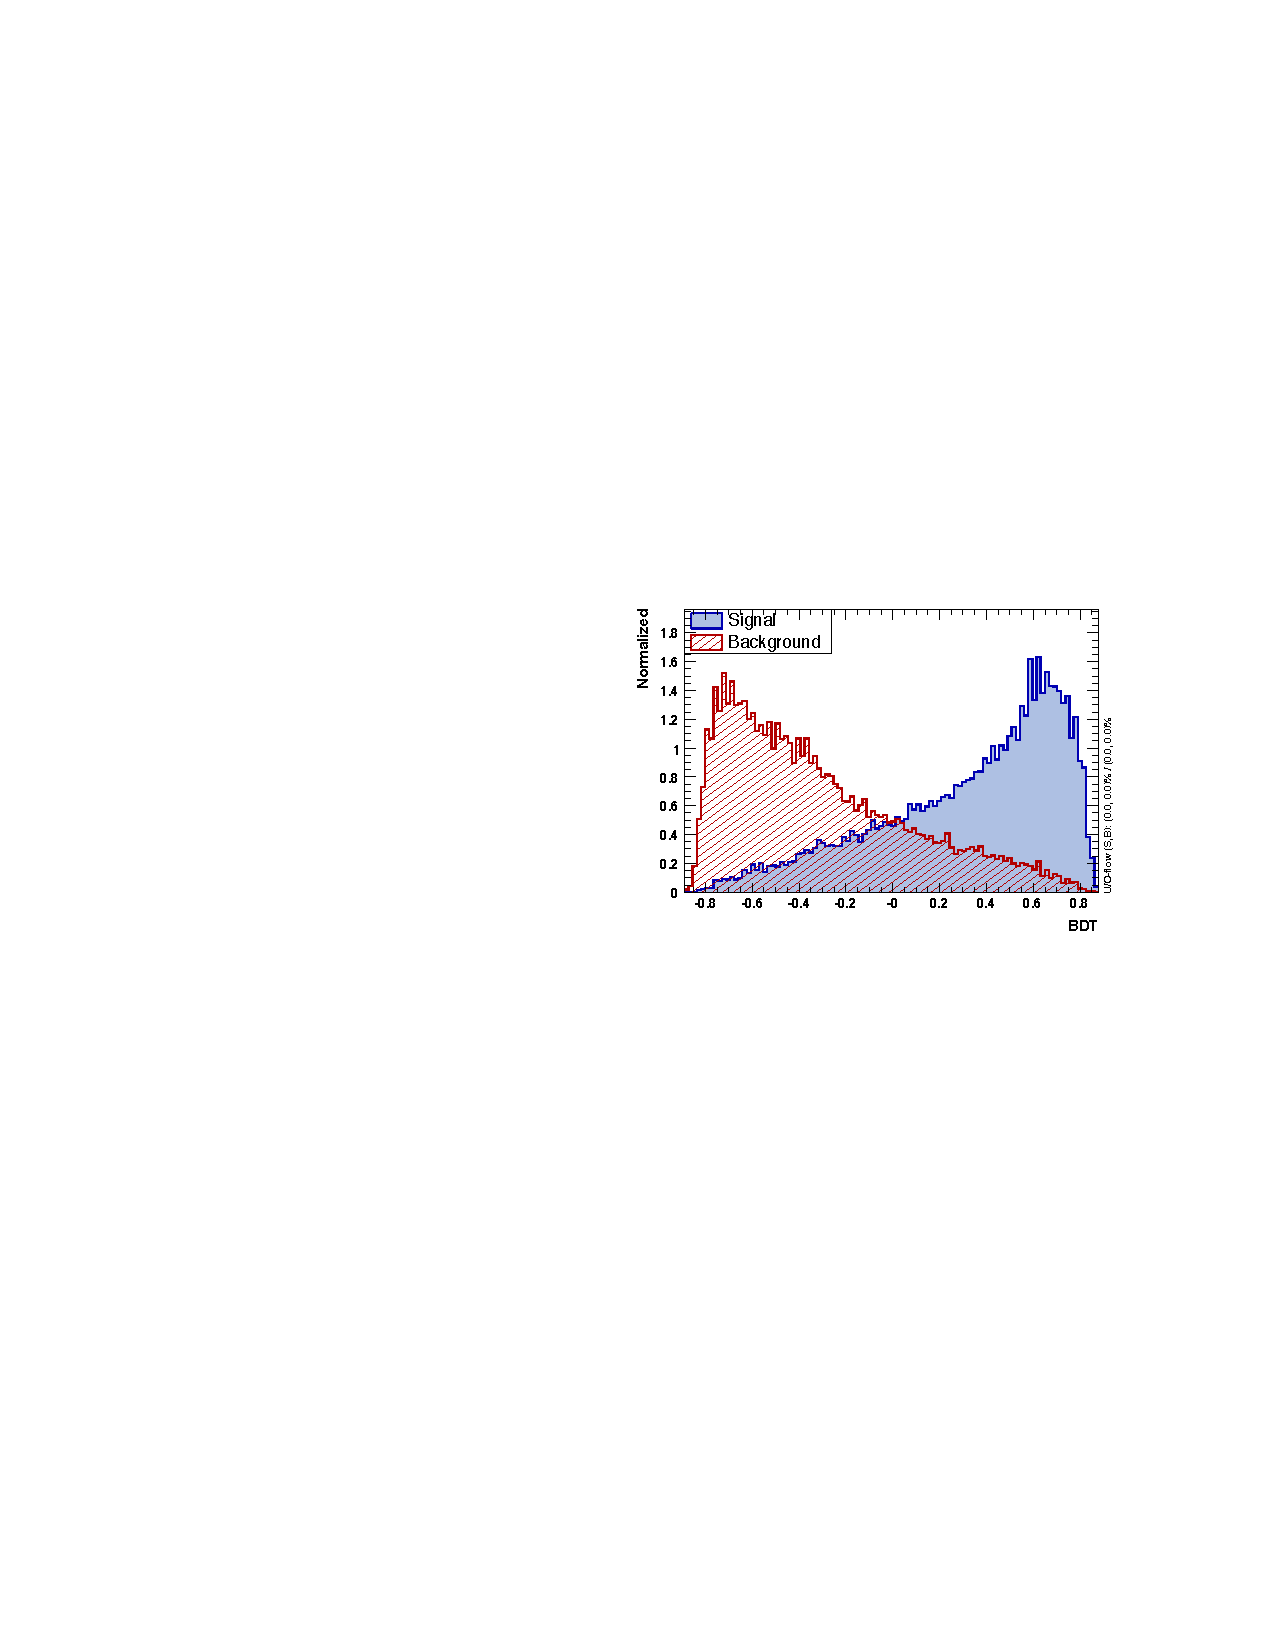
\includegraphics[height=1.7in]{example-TMVA-BDT.pdf}
 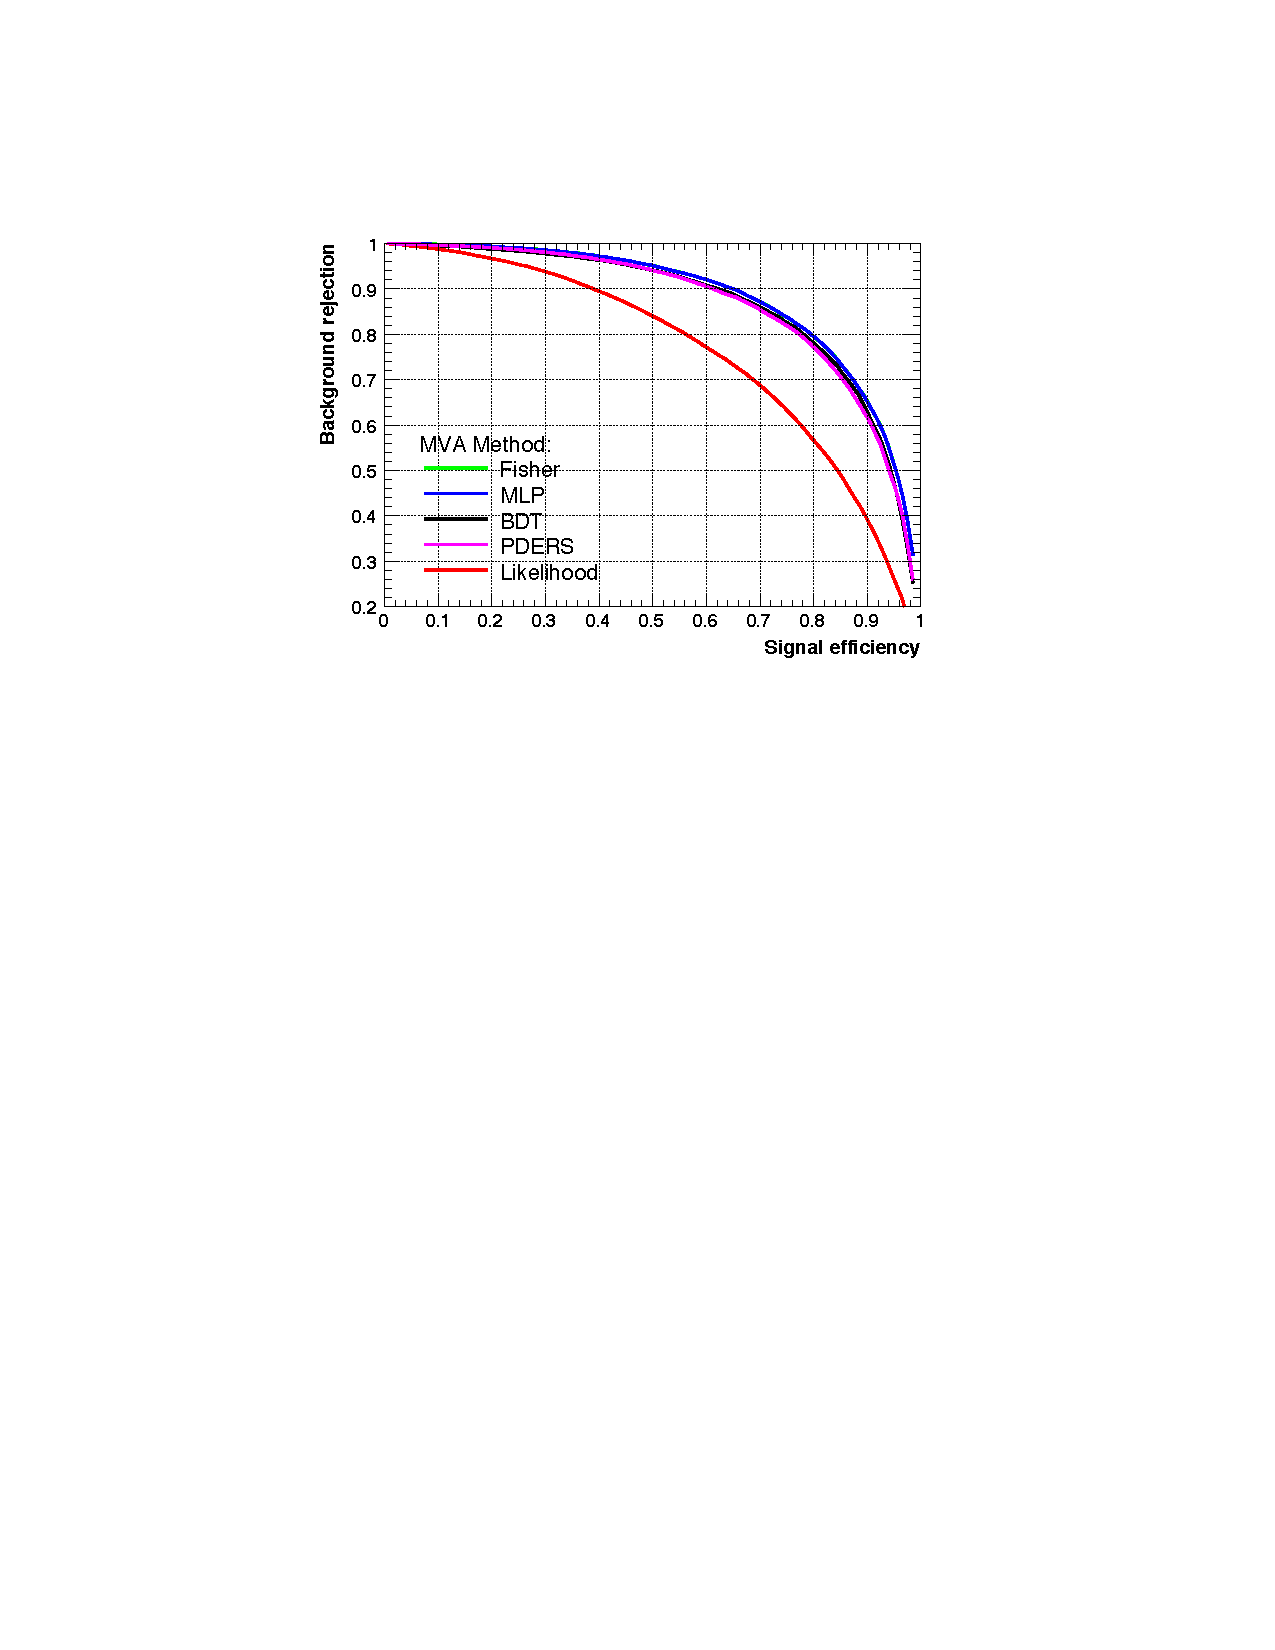
\includegraphics[height=1.7in]{example-TMVA-ROC.pdf}
\caption{Left: an example of the distributions $p_b(\hat s|\nu)$ and $p_s(\hat s|\nu)$ when the classifier $s$ is a boosted-decision tree (BDT). Right: the corresponding ROC curve (right) for this and other classifiers. (Figures taken from TMVA manual.)}
\label{fig:tmva}
\end{center}
\end{figure}
%\bigskip

These steps feed into a subsequent statistical test based on the observed data 
${D=(x_1, \dots, x_n)}$. For each event, the classifier is evaluated and one performs inference on a parameter $\mu$ related to the presence of the signal contribution. In particular, one forms the statistical model\footnote{Sometimes there is an additional Poisson term when expected number of signal and background events is known, which is referred to as an extended likelihood or marked Poisson model.} 
\begin{equation}\label{eq:typicalML}
p( D \,|\, \mu, \nu) = \prod_{e=1}^n \, \left[\, \mu \hat{p}_s( \hat s(x_e) \, |\,  \nu)  + (1-\mu)\, \hat{p}_b( \hat s(x_e) \,|\, \nu) \,\right] \; .
\end{equation}
%where $\mu=0$ is the null (background-only) hypothesis and $\mu>0$ is the alternate (signal-plus-background) hypothesis.\footnote{Sometimes there is an additional Poisson term when expected number of signal and background events is known, which is referred to as an extended likelihood.} 
%Typically, we are interested in inference on $\mu$ and $\nu$ are nuisance parameters.

\subsection{Comments on typical usage of machine learning in HEP}

Nuisance parameters are an after thought in the typical usage of machine learning in HEP. In fact, most discussions would related to the training and optimizing the classifier only consider $p_b(x)$ and $p_s(x)$ with $\nu=\nu_0$ being implicit. However, as experimentalists we know that we must account for various forms of systematic uncertainty, parametrized by nuisance parameters $\nu$. In practice, we take the classifier as fixed and then propagate uncertainty through the classifier as in Eq.~\ref{eq:typicalML}. Building the distribution $p(\hat s|\nu)$ for values of $\nu$ other than the nominal $\nu_0$ used to train the classifier can be thought of as a calibration necessary for classical statistical inference; however, this classifier is clearly not optimal for $\nu \ne \nu_0$.

\subsection{A more powerful  approach}

The standard use of machine learning in HEP can be improved by training a parametrized, discriminative classifier corresponding to the generalized likelihood ratio test 
\begin{equation}
\lambda(\mu) = \frac{p(D|\mu, \hat{\hat{\nu}})}{p(D|\hat \mu, {\hat{\nu}})} \;,
\end{equation}
following the approach outlined in Section~\ref{S:GLR}. 

There is an interesting distinction between this approach and the standard use in which the classifier is trained for a fixed $\nu_0$. In the standard use one trains a classifier for signal vs. background, which is equivalent (in an ideal setting) to training a classifier for  null (background-only) vs. alternate (signal-plus-backgound) since the resulting regression functions are one-to-one with each other.
% as 
%\begin{equation}
% \frac{p(x| 0, \nu_0)}{p(x|\hat \mu, \nu_0)} =  \frac{p_b(x| \nu_0)}{ \mu p_s( x_e \, |\,  \nu_0)  + (1-\mu)\, p_b( x_e \,|\, \nu_0)} = \left[ c_1 + c_2   \frac{p_s(x| \nu_0)}{ p_b( x_e \,|\, \nu_0)} \right ]^{-1} \; ,
%\end{equation}
%and $c_1$ and $c_2$ are constants. Specifically, the two  likelihood ratios are in one-to-one correspondence, so an ideal algorithm would lead to equivalent tests. 
In contrast, in the case of the generalized likelihood ratio test 
\begin{equation}\label{eq:hep_improved}
 \frac{p(x| 0, \hat{\hat{ \nu}})}{p(x|\hat \mu, \hat\nu)} =  \frac{p_b(x| \hat{\hat{ \nu}})}{ \hat \mu p_s( x_e \, |\,  \hat\nu)  + (1- \hat \mu )\, p_b( x_e \,|\, \hat \nu)} \; ,
\end{equation}
the background components don't cancel and there is an additional term $p_b(x| \hat{\hat{ \nu}})/p_b(x| {\hat{ \nu}})$.
In practice, with classifiers of finite capacity, there will be some tradeoff between taking into account this additional term and the more challenging learning problem when $\mu$ is very small. 

\subsection{Decomposing tests between mixture models into their components}

In this section we generalize the capacity focusing technique of training classifiers to discriminate between components of a mixture model. First, we generalize Eq.~\ref{eq:hepGen} to a mixture model of several components
\begin{equation}
p(x|\theta)=\sum_c w_c(\theta) p_c(x| \theta) \;.
\end{equation}
%In the case of particle physics, the distributions $p(x|\theta)$ is not a Gaussian Mixture Model, but mixture of  complicated distributions associated to relatively few types of particle interactions. Moreover, when searching for a new particle, the null hypothesis would correspond to some of the coefficients $w_c=0$ while the alternate ``signal-plus-background'' hypothesis would have $0<w_{c\in \rm signal} \ll w_{c\in \rm background}$. In some cases $w_{c\in \rm signal} / w_{c\in \rm background} <10^{-6}$, which means the alternate hypothesis is a small perturbation to the null hypothesis. This can be a challenge for typical classifiers because they should devote their capacity to the region where $p_{c\in \rm signal}(x) / p_{c\in \rm background}(x)$ is relatively large. Lastly, even when the distributions $p_c(x|\theta)$ are well known, it is often the case that the coefficients are uncertain or treated as completely unknown. These all present challenges to machine learning algorithms that aim to learn $s(x; \theta_0, \theta_1)$.
%
%\begin{equation}
%\frac{p(x|\theta_0)}{p(x|\theta_1)}= \frac{\sum_c w_c(\theta_0) p_c(x| \theta_0)}{\sum_c w_c(\theta_1) p_c(x| \theta_1)} 
%\end{equation}
%
%\begin{equation}
%\frac{p(x|\theta_0)}{p(x|\theta_1)}= \sum_c \frac{ w_c(\theta_0) p_c(x| \theta_0)}{\sum_{c'} w_{c'}(\theta_1) p_{c'}(x| \theta_1)} 
%\end{equation}
%
It is possible to re-write the target likelihood ratio between two mixture models in terms of pairwise classification problems. 
\begin{eqnarray}\label{eq:decompose}
\frac{p(x|\theta_0)}{p(x|\theta_1)} & =& \frac{\sum_c w_c(\theta_0) p_c(x| \theta_0)}{\sum_{c'} w_{c'}(\theta_1) p_{c'}(x| \theta_1)} 
\\
%&=& \sum_c \frac{ w_c(\theta_0) p_c(x| \theta_0)}{\sum_{c'} w_{c'}(\theta_1) p_{c'}(x| \theta_1)} \\
%&=& \sum_c \left[ \frac{\sum_{c'} w_{c'}(\theta_1) p_{c'}(x| \theta_1)}{ w_c(\theta_0) p_c(x| \theta_0)}  \right]^{-1} \\
&=& \sum_c \left[ \sum_{c'} \frac{ w_{c'}(\theta_1)}{w_c(\theta_0)} \frac{ p_{c'}(x| \theta_1)}{  p_c(x| \theta_0)}  \right]^{-1} \\ \label{eq:decomposedResult}
&=& \sum_c \left[ \sum_{c'} \frac{ w_{c'}(\theta_1)}{w_c(\theta_0)} \frac{ p_{c'}(s_{c,c',\theta_0, \theta_1}| \theta_1)}{ p_c(s_{c,c',\theta_0, \theta_1}| \theta_0)}  \right]^{-1} 
\end{eqnarray}
The second line is a trivial, but useful decomposition into pair-wise classification between $p_{c'}(x|\theta_1)$ and $p_c(x|\theta_0)$.  The third line uses Theorem~1 to relate the high-dimensional likelihood ratio into an equivalent calibrated likelihood ratio based on the univariate density of the corresponding classifier, denoted $s_{c,c',\theta_0, \theta_1}$. In the situation where the only free parameters of the mixture model are the coefficients $w_c$, then the distributions $p_{c}(s_{c,c',\theta_0, \theta_1}| \theta)$ are independent of $\theta$ and can be pre-computed (after training the discriminative classifier, but before evaluating the  likelihood ratio). Equation~\ref{eq:decomposedResult} allows one to take advantage of both the parametrized classifier as in Eq.~\ref{eq:hep_improved} and the capacity focusing technique in the typical HEP usage pattern. 


%
%The idea here is to combine the calibration of the distributions of the classifier output and a more optimal family of classifiers $\hat s(x; \nu_0, \nu_1)$. Creating the family of classifiers is straight forward, one simply augments the training data with $x$ examples drawn from several values of $\nu$ and then includes the corresponding value of $\nu$ as an input to the classifier. Thus $\{x_e,c_e\} \to \{x_e,\nu_{0,e},\nu_{1,e}, c_e\}$ leading to a parametrized learner $\hat s(x)\to \hat s(x;\nu_0, \nu_1)$. This leads to a complication: one does not know the value of $\nu$ to use when evaluating the parametrized classifier $\hat s(x;\nu_0, \nu_1)$, so one cannot simply pre-compute $\hat s_e$ before performing the likelihood fit.  However, when performing a likelihood ratio test, one can calculate the maximum likelihood estimate and conditional maximum likelihood estimate according to Eq.~\ref{eq:mle} and then form the equivalent likelihood ratio test according to Eq.~\ref{eq:equivLRtest}. 


%Equivalently, once one has determined $\hat{\theta}$ and $\hat{\hat{\theta}}$, then one can specify the parameters of the mapping $s(x;\hat{\hat{\theta}}, \hat{\theta})$ and then following Eq.~\ref{eq:NP} form the likelihood
%\begin{equation}\label{eq:parametrizedML}
%p( D \,|\, \mu, \nu) = \prod_{e=1}^n \, \left[\, \mu p_s( s(x_e;\nu_0, \nu_1) \, |\,  \nu)  + (1-\mu)\, p_b( s(x_e;\nu_0, \nu_1) \,|\, \nu) \,\right] \; ,
%\end{equation}
%which is a natural generalization of Eq.~\ref{eq:typicalML}.

%The construction in Eq.~\ref{eq:parametrizedML} presents a computational challenge as for each value of $\nu$ one has a new mapping $s: x\to\mathbb{R}$. The most naive realization of this would be to generate synthetic data $\{x_e\}$ according to $p_c(x|\nu)$, evaluate $s(x_e ; \nu_0, \nu_1)$, and then use a histogram, kernel density, or other non-parametric density estimation procedure to estimate $p_c( s | \nu)$. This approach is not realistic in situations where $p_c(x|\nu)$ is realized with expensive computer simulations; thus, some interpolation strategy or emulator over a fixed set of parameter points $\{\nu_i\}$ would typically be used.

\subsection{Measuring particle properties}

While the original motivation for this work was to improve the treatment of systematic uncertainties in new particle searches by parametrizing the classifier in terms of the nuisance parameters $\nu$, the same approach can be used to for parameter inference. In the case of new particle searches the parameter of interest is the mixture coefficient for the signal component $p_s(x|\nu)$. When measuring particle properties the distribution of the features also depend on parameters such as a particle's mass and quantum numbers. This is easily accommodated by extending $p_s(x|\nu) \to p_s(x|\theta)$, where $\theta$ includes both parameters of interest and nuisance parameters. 

This formalism represents is a significant step forward in the usage of machine learning in HEP, where classifiers have always been used between two static classes of events and not parametrized explicitly in terms of the physical quantities we wish to measure. The work of  ~\citek{Whiteson:2006ws} is the closest example as the stochastic optimization was directly trying to minimize the measurement uncertainty of a particle's mass; however, the resulting classifier was fixed. This approach also offers the advantage that it explicitly reformulates the per-experiment optimization to the per-event optimization, which is less computationally intensive.

Another approach that is similar in spirit is the so-called matrix element method, in which one  directly computes an approximate likelihood ratio by performing a computationally intensive integral associated to the detector response~\citek{Volobouev:2011vb}. In the approach considered in this paper, the detector response is naturally handled by the Monte Carlo sampling used in the simulation of the detector; however, that integral is intractable for the matrix element method. Even with drastic simplifications of the detector response, the matrix element method can take several minutes of CPU time per event to calculate the likelihood ratio $q(x)$. The work here can be seen as aiming at the same conceptual target, but utilizing machine learning to overcome the complexity of the detector simulation. It also offers enormous speed increase for evaluating the likelihood at the cost of an initial training stage. In practice, the matrix element method has only been used for searches and measurement of a single physical parameter (sometimes with a single nuisance parameter as in~\citek{Aaltonen:2010yz}).

Contemporary examples where the technique presented here could have major impact on HEP include the measurement of coefficients to quantum mechanical operators describing the decay of the Higgs boson~\citek{Chen:2014pia} and, if we are so lucky, measurement of the mass of supersymmetric particles in cascade decays~\citek{Allanach:2000kt}.  Both of these examples involve data sets with many events, each with a feature vector $x$ that has on the order of 10 components, and a parameter vector $\theta$ with 5-10 parameters of interest and possibly many more nuisance parameters. 
%The state of the art approaches for supersymmetric particle masses typically involve high-level features engineered based on physics intuition
%Many approaches have been tried for measuring supersymmetric particle masses, often based on event level features engineered based on physics intuition and varying 
The state of the art for the operator coefficients of the Higgs decay uses the so-called matrix element likelihood analysis (MELA) in which the equivalent of $s(x; \theta_0, \theta_1)$ is approximated by neglecting detector effects~\citek{Bolognesi:2012mm}. 

\bigskip

\subsection{Related work}\label{S:Related}

%Refs to include:
%\citek{ClaytonScott,AndrewY.Ng,SamT.Roweis,EricP.Xing,SujaySanghavi,BiancaZadrozny,Zadrozny2001,}

\cite{ClaytonScott} and \cite{JMLR:v14:tong13a} consider the machine learning problem associated to Neyman-Pearson hypothesis testing. As in this work, they consider the situation where one does not have access to the underlying distributions, but only has i.i.d. samples from each hypothesis. This work generalizes that goal from the Neyman-Pearson setting to generalized likelihood ratio tests and emphasizes the connection with classification. Perhaps a  formal treatment similar to the Neyman-Pearson case can be brought to bear in this more general setting.
\cite{TommiJaakkola} explore a way of leveraging generative models to derive kernel functions for use in discriminative methods. This interesting work is distinct from the point made here in which the generative model is being used for the purpose of providing training data and calibration.  
%\cite{McCallum} consider a hybrid generative/discriminative classifier; however, the goal of that work is not to leverage a generative model for the data, but to use both approaches to learn different subsets of the parameters in a single hybrid classifier.  
\cite{BiancaZadrozny} emphasize the importance of calibrated probability estimates from decision trees and naive Bayesian classifiers and investigate various approaches to achieve this. In contrast to that work, we are not interested in calibrated probability estimates for $p(y|x)$ for individual events, but instead we use the calibration to correct for non-linear transformations of the target likelihood ratio and, perhaps, to provide calibrated p-values based on those likelihood ratio tests. \cite{Ihler2004} take on a different problem (tests of statistical independence) by using machine learning algorithms to find  scalar maps from the high-dimensional feature space that achieve the desired statistical goal when the fundamental high-dimensional test is intractable.

\cite{Neal:2007zz} also considered the problem of approximating the likelihood function when only a generative model is available. That work sketches a scheme in which one uses a classifier with both $x$ and $\theta$ as an input to serve as a dimensionality reduction map. 
The key distinction comes in the handling of $\theta$.  Neal says  ``we cannot use the classifier on real data, since we don't know the correct value for [$\theta]$'' and goes on to outline an approach where one uses regression on a per-event basis to estimate $\hat{\theta}(x)$ and perform the composition $s(x; \hat{\theta}(x))$ (much like profiling).\footnote{Neal considers a lower-dimensional `bottlenecks' $\theta^*=g(\theta)$, which are not essential to the discussion here.}  This can lead to a significant loss of information since (at least in most particle physics examples) a single event carries little information about the true value of $\theta$, though the full data set $D$ may be informative -- for instance, a single observation would not be sufficient to estimate the variance of a distribution, though repeated observations would.  The work of Neal correctly identifies this as an approximate procedure even in the case of a ideal classifier. In contrast, the approach described here does not eliminate the dependence of the classifier on $\theta$.%
\footnote{As a technical point, in Neal's work, the focus is on approximating the likelihood function (up to a multiplicative constant), which is equivalent to evaluating the ratio  with respect to a fixed $\theta_1$ as in Eq.~\ref{eq:mle_withs}. In Neal's case, the dependence on $\theta$ is eliminated via $s(x; \hat{\theta}(x))$ and the map is constant; however, in this approach the map ratio is explicitly parametrized in terms of $\theta$, so the ratio is important for canceling the corresponding Jacobian factors.} Instead, we embed a parametrized classifier into the likelihood and postpone the evaluation of the classifier to the point of evaluation of the likelihood when $\theta$ is explicitly being tested. This avoids the loss of information that occurs from the regression step $\hat{\theta}(x)$ proposed by Neal and leads to Theorem~1, which is an exact result in the case of an ideal classifier. 


\section{Conclusions}

We have outlined a technique to reformulate generalized likelihood ratio test over a high-dimensional data set with multiple events in terms of a univariate density of a classifier score. 
We have shown that a parametrized family of discriminative classifiers $s(x; \theta_0, \theta_1)$ trained and calibrated with a simulator  $p(x|\theta)$ can be used to approximate the  likelihood ratio  $\prod_i p(x_i|\theta_0)/p(x_i|\theta_1)$ even when it is not possible to directly evaluate the likelihood $p(x|\theta)$.   This approach leverages the power of machine learning in a classical statistical setting. It offers an alternative to approximate Bayesian computation for parameter inference in the likelihood-free setting that can also be used in the frequentist formalism without specifying a prior over the parameters. 

%Furthermore, this allows one to turn the optimization of the procedure for the per-experiment test into optimization of a per-event classification problem and a calibration procedure.

%In particular, it extends the common usage of machine learning for simple hypothesis testing to include the parameter estimation, confidence intervals, and composite hypothesis testing.

%We have shown that a parametrized family of discriminative classifiers $s(x; \theta_0, \theta_1)$ trained and calibrated with a generative model $p(x|\theta)$ can be used to approximate statistical inference likelihood based on the  ratio $p(x|\theta_0)/p(x|\theta_1)$ when it is not possible to evaluate the densities $p(x|\theta)$ for an arbitrary $x$. 


%\section{Possible Extensions}
%The approach describe thus far has been agnostic as to the type of classifier used to produce $s(x)$ and $s(x; \nu)$. In practice, we have used standard packages for the training of these learners. In particular, the loss function for these learning algorithms is based on classification performance of individual $(x_e, c_e)$ feature $\to$ target examples. However, in overarching statistical procedure that uses the statistical model in Eq.~\ref{eq:typicalML} or \ref{eq:parametrizedML} the quantity we wish to optimize is a property of an entire data set $\{x_e\}$ or ensembles of data sets that can be generated from the statistical models $p_c(x|\theta)$. 
%
%For example, in typical hypothesis testing problems posed in the Neyman-Pearson context one would be interested in minimizing type II error under a fixed rate of typeI error rate. In the presence of systematic uncertainty and nuisance parameters, the loss function may become more complicated. The recent Higgs boson machine learning challenge hosted by Kaggle, the evaluation was the approximate median significance (AMS) that characterized the power of a hypothesis test between $\mu=0$ (the background only hypothesis) and $\mu=\mu_0$ (the signal+background hypothesis, where $\mu_0$ is a small number reflecting the small Higgs signal that would be found in addition to the much larger background process) in the presence of uncertainty on the background normalization. 
%Interestingly, the top entries to the challenge did not improve by focusing on this alternative loss function 
%in training their classifier, but instead used it for the optimization of a threshold on the score (a working point on the ROC curve) that was related to the way the challenge was designed. This suggests that the standard 
%classification loss functions lead to similar optimizations and that refinements for the custom loss functions
%are not easy to come by.
%
%More generally, there is an avenue of research associated to custom loss functions specifically designed 
%for these real world statistical problems. One direction might be to choose loss functions that make 
%some balance between the standard classification loss, take into account robustness with respect to nuisance parameters, and population-level quantities like type I and II error.
%
%\subsection{A different starting point}
%
%Instead of evolving from the traditional usage of ML in HEP, let's start from scratch with $p_c(x|\theta)$ and a well defined objective.  
%
%\subsubsection{Simple Hypothesis Testing}
%
%Consider the situation of simple hypothesis testing between the background-only $\mu=0$ and signal+background hypothesis $\mu=\mu_0=\nu_s/(\nu_s+\nu_b)$ for $\theta=\theta_0$.  Let us assume that not only can we use the $p_c(x|\theta_0)$ as a generative model, but that we can evaluate the probability density at any point $x$.  The statistical model is given by
%\begin{equation}\label{eq:NP}
%p( D \,|\, \mu, \theta) = \prod_{e=1}^n \, \left[\, \mu p_1( x_e \, |\,  \theta)  + (1-\mu)\, p_b( x_e \,|\, \theta) \,\right] \; .
%\end{equation}
%The objective is to find a  test statistic $T(D)$ (a map from the space of the data to $\mathbb{R}$)  
%and a threshold $k_\alpha$ that minimizes the rate of type-II error (i.e. $P(T(D) < k_\alpha | \mu=\mu_0, \theta_0) = \beta$ under the constraint of a fixed rate of type-I error ( i.e.  $P(T(D) > k_\alpha | \mu=0, \theta_0) = \alpha$ ).
%The Neyman-Pearson lemma states that the optimal test statistic is the likelihood ratio, or equivalently, the log-likelihood ratio 
%\begin{equation}
%T =  \log \frac{p(D | \mu=\mu_0, \theta_0)}{p(D | \mu=0, \theta_0)}
%\end{equation}
%When the $x_e$ are i.i.d., then the log-likelihood ratio expands into a sum
%\begin{equation}
%T =   \sum_{e=1}^n \underbrace{\log \left[ 1+c_1\frac {p_1(x_e | \theta_0) }{ p_b(x_e | \theta_0) } \right]}_{q(x_e)} + c_2\;,
%\end{equation}
%where $c_1=\mu/(1-\mu)$ and $c_2=\lop(1-\mu)$ are constants for the simple hypothesis test.
%
%Here we see that the optimal $T$ for the experiment is composed of a sum over events of a linear linear function of the per-event function $q(x)$. A monotonic, but non-linear function of $q(x)$ would not lead to an equivalent hypothesis test. 
%
%The important part of the per-event function $q(x)$ is that it defines contours in the feature space $x$. These contours are also equivalent to the function $p_1(x|\theta_0)/p_b(x|\theta_0)$, the signal-to-background ratio. If we can find a machine learner $s(x)$ that is a monotonic function of $p_1(x|\theta_0)/p_b(x|\theta_0)$ it will share the same contours. Then the remaining challenge is to find the appropriate rescaling that gives back  linear function $q(x)$. 
%
%\textbf{Postulate:}
%\begin{equation}
%T' = \sum_{e=1}^n \underbrace{\log \left[ 1+c_1\frac {p_1(s(x_e) | \theta_0) }{ p_b(s(x_e) | \theta_0) } \right]}_{q(s_e)} \;,
%\end{equation}
%leads to an equivalent test, where $s_e \equiv s(x_e)$
%\begin{equation}
%p_c(s) = \int dx \, \delta(s-s(x)) \, p_c(x)  \,  |\partial s / \partial x|^{-1}
%\end{equation}
%
%
%
%Note, in order to form the hypothesis test, one still needs to build the build the $p_0(T|\theta)$ to calibrate the threshold  $T>k_\alpha$ that gives rise to a test of size $\alpha$. 
%
%
%
%\textbf{Proof (in progress):}
%
%We want to show density is the same 
%
%\begin{equation}
%p_c(q_x) = \int dx \delta(q_x-q_x(x)) p_c(x) / |\partial q_x / \partial x|
%\end{equation}
%
%\begin{equation}
%p_c(q_s) = \int dx \delta(q_s-q_s(s(x))) \, p_c(x) \, / |\partial q_s / \partial x|
%\end{equation}
%sufficient to show $q(x_e) = q(s(x_e))$.  Here we use that $p_1(x)/p_0(x)=\textrm{const}$ for all points on the level-set $\Omega_c$ given by $ \delta(c-s(x))$. 
%\begin{equation}
%\frac {p_1(c | \theta_0) }{ p_0(c | \theta_0) } = 
%\frac { \int dx \delta(c-s(x)) \, p_1(x_e | \theta_0) }{ \int dx \delta(c-s(x)) \, p_0(x | \theta_0)  } = 
%\frac {c \int dx \delta(c-s(x)) \, p_0(x | \theta_0)  }{ \int dx \delta(s-s(x)) \, p_0(x | \theta_0)  } = c =\frac {p_1(x | \theta_0) }{ p_0(x | \theta_0) } 
%\end{equation}
%
%
%
%%\begin{equation}
%%p_c(q_s) = \int ds \delta(q_s-q_s(s)) \,p_c(s) \, / |\partial q_s / \partial s|
%%\end{equation}
%
%
%This is the test statistic that one would naturally get from constructing the likelihood function for the 1-d distributions of the output of the machine learner
%\begin{equation}\label{eq:NP}
%p( \{s_e\} \,|\, \mu, \theta) = \prod_{e=1}^n \, \left[\, \mu p_1( s_e \, |\,  \theta)  + (1-\mu)\, p_0( s_e \,|\, \theta) \,\right] \; .
%\end{equation}
%Thus this motivates Eq.~\ref{eq:typicalML} in the more general case. 
%
%
%Question:
%Where does this fit in:
%\begin{equation}
%T'' = \sum_{e=1}^n \underbrace{ \log \left[ 1+c_1 s(x_e) \right] }_{q'(s_e)} \;,
%\end{equation}
%
%
%
%Usefulness:
%If we can readily compute $p_c(x|\theta_0)$, then there would be no need for machine learning algorithms. However,  these densities are often difficult to compute though one can readily use them as a generative model to produce samples. In that case, one might wish to use a machine learning algorithm to find $s(x) \approx p_1(x|\theta_0) / p_0(x|\theta_0)$. 
%
%Conclusion, while it is possible to start directly with the Neyman-Pearson loss function of type-II error under the constraint of fixed size and try to find a per-experiment learner $T(D)$, it is more convenient to cast the problem in terms of learning a per-event function $s(x)$, and then calibrate it to be a linear function of $q(x)$.
%
%\newpage
%
%Given $x\in \mathbb{R}^n$ and two smooth, real-valued functions $p_1(x)$ and $p_0(x)$ define 
%\begin{equation} 
%s(x)=\frac{p_1(x)}{p_2(x)}
%\end{equation}.
%Define $p_1(c) = \int dx \delta(c - s(x) ) \, p_1(x)$ and $p_0(c) = \int dx \delta(c - s(x) ) \, p_0(x)$.
%I wish to show
%\begin{equation}
%\frac{p_1(c)}{p_0(c)} = \frac{p_1(x)}{p_0(x)}
%\end{equation}
%$\forall x \ni s(x)=c$.
%
%Sketch of Proof: 
%let $\Omega_{c}$ be the level set $\{x \mid s(x) = c \}$ and $\hat{n}=\nabla s(x) / |\nabla s(x)|$ be the perpendicular direction to the surface at the point $x$. The  coordinate perpendicular to $\Omega$ can be written $y = x+\epsilon \hat{n}$. In these coordinates, the integral $\int dx \to \int d\Omega d\epsilon$, thus
%\begin{equation}
%p_1(c) = \int dx \delta(c-s(x)) p_1(x) = \int d\Omega p_1(x) / |\partial s(x)/\partial \epsilon|
%\end{equation}
%Similarly for $p_0(c)$. We can factor out of the integral $s(x)=p_1(x)/p_0(x)$ since it is constant over $\Omega$.
%Thus
%\begin{equation}
%p_1(c) = \int dx \delta(c-s(x)) p_1(x) = \int d\Omega p_1(x) / |\partial s(x)/\partial \epsilon| = s(x) \int d\Omega p_0(x) / |\partial s(x)/\partial \epsilon|
%\end{equation}
%and we arrive at the result
%\begin{equation}
%\frac{p_1(c)}{p_0(c)} = \frac{s(x) \int d\Omega p_0(x) / |\partial s(x)/\partial \epsilon|}{ \int d\Omega p_0(x) / |\partial s(x)/\partial \epsilon|} = \frac{p_1(x)}{p_0(x)} \;.
%\end{equation}
%
%
%
%
%\subsection{misc notes}
%
%
%
%
%The distribution of $s$ is fully determined by the mapping $s(x_e; \theta_0, \theta_1)$ and the distribution $p(x)$, which we can write
%\begin{equation}
%p(s_e) = \int dx \, \delta(s_e-s(x)) \, p(x)  \; .
%\end{equation}
%\textbf{NEED Jacobian for x $\to$ s independent of delta function part, or double counting?}
%
%
%\textbf{Theorem 1:}
%Let $\Omega_{c}$ be the level set $\{x \mid s(x) = c \}$ and $\hat{n}=\nabla s(x) / |\nabla s(x)|$ be the orthonormal vector to the surface at the point $x$. The component perpendicular to $\Omega_c$ can be written $x+\epsilon \hat{n}$. In these coordinates, we rewrite integral $\int dx \to \int d\Omega_c d\epsilon$, thus
%\begin{equation}
%p_1(c) = \int dx \delta(c-s(x)) p_1(x) = \int d\Omega_c p_1(x)  / | \hat{n} \cdot \nabla q_s  |
%\end{equation}
%Similarly for $p_0(c)$. We can factor out of the integral $s(x)=p_1(x)/p_0(x)$ since it is constant over $\Omega_c$.
%Thus
%\begin{equation}
%p_1(c) = \int dx \delta(c-s(x)) p_1(x) = \int d\Omega p_1(x) / |\partial s(x)/\partial \epsilon| = s(x) \int d\Omega p_0(x)  / | \hat{n} \cdot \nabla q_s  |
%\end{equation}
%and we arrive at the result
%\begin{equation}
%\frac{p_1(c)}{p_0(c)} = \frac{s(x) \int d\Omega p_0(x) / |\partial s(x)/\partial \epsilon|}{ \int d\Omega p_0(x) / |\partial s(x)/\partial \epsilon|} = \frac{p_1(x)}{p_0(x)} \;\hspace{3em} \forall x\in\Omega_c.
%\end{equation}
%
%
%
%
%
%Define $p_1(c) = \int dx \delta(c - s(x) ) \, p_1(x)$ and $p_0(c) = \int dx \delta(c - s(x) ) \, p_0(x)$.
%I wish to show
%\begin{equation}
%\frac{p_1(c)}{p_0(c)} = \frac{p_1(x)}{p_0(x)}
%\end{equation}
%$\forall x \ni s(x)=c$.
%
%
%Given $x\in \mathbb{R}^n$ and two smooth, real-valued functions $p_1(x)$ and $p_0(x)$ define 
%\begin{equation} 
%s(x)=\frac{p_1(x)}{p_0(x)}
%\end{equation}.
%Define $p_1(c) = \int dx \delta(c - s(x) ) \, p_1(x)$ and $p_0(c) = \int dx \delta(c - s(x) ) \, p_0(x)$.
%I wish to show
%\begin{equation}
%\frac{p_1(c)}{p_0(c)} = \frac{p_1(x)}{p_0(x)}
%\end{equation}
%$\forall x \ni s(x)=c$.
%
%Sketch of Proof: 
%let $\Omega_{c}$ be the level set $\{x \mid s(x) = c \}$ and $\hat{n}=\nabla s(x) / |\nabla s(x)|$ be the perpendicular direction to the surface at the point $x$. The  coordinate perpendicular to $\Omega$ can be written $y = x+\epsilon \hat{n}$. In these coordinates, the integral $\int dx \to \int d\Omega d\epsilon$, thus
%\begin{equation}
%p_1(c) = \int dx \delta(c-s(x)) p_1(x) = \int d\Omega p_1(x) / |\partial s(x)/\partial \epsilon|
%\end{equation}
%Similarly for $p_0(c)$. We can factor out of the integral $s(x)=p_1(x)/p_0(x)$ since it is constant over $\Omega$.
%Thus
%\begin{equation}
%p_1(c) = \int dx \delta(c-s(x)) p_1(x) = \int d\Omega p_1(x) / |\partial s(x)/\partial \epsilon| = s(x) \int d\Omega p_0(x) / |\partial s(x)/\partial \epsilon|
%\end{equation}
%and we arrive at the result
%\begin{equation}
%\frac{p_1(c)}{p_0(c)} = \frac{s(x) \int d\Omega p_0(x) / |\partial s(x)/\partial \epsilon|}{ \int d\Omega p_0(x) / |\partial s(x)/\partial \epsilon|} = \frac{p_1(x)}{p_0(x)} \;.
%\end{equation}
%
%
%
%
%
%
%
%Note, in order to form the hypothesis test, one still needs to build the build the $p_0(T|\theta)$ to calibrate the threshold  $T>k_\alpha$ that gives rise to a test of size $\alpha$. 
%
%
%
%\textbf{Proof (in progress):}
%
%We want to show density is the same 
%
%\begin{equation}
%p(q_x|\theta) = \int dx \delta(q_x-q_x(x)) p(x|\theta)  / | \hat{n} \cdot \nabla q_s  |
%\end{equation}
%
%\begin{equation}
%p(q_s|\theta) = \int dx \delta(q_s-q_s(s(x))) \, p(x|\theta) \, / | \hat{n} \cdot \nabla q_s  |
%\end{equation}
%sufficient to show $q(x_e) = q(s(x_e))$.  Here we use that $p_1(x)/p_0(x)=\textrm{const}$ for all points on the level-set $\Omega_c$ given by $ \delta(c-s(x))$. 
%\begin{equation}
%\frac {p_1(c | \theta_0) }{ p_0(c | \theta_0) } = 
%\frac { \int dx \delta(c-s(x)) \, p_1(x_e | \theta_0) }{ \int dx \delta(c-s(x)) \, p_0(x | \theta_0)  } = 
%\frac {c \int dx \delta(c-s(x)) \, p_0(x | \theta_0)  }{ \int dx \delta(s-s(x)) \, p_0(x | \theta_0)  } = c =\frac {p_1(x | \theta_0) }{ p_0(x | \theta_0) } 
%\end{equation}
%
%
%
%%\begin{equation}
%%p_c(q_s) = \int ds \delta(q_s-q_s(s)) \,p_c(s) \, / |\partial q_s / \partial s|
%%\end{equation}
%
%



\section*{Acknowldgements}
KC would like to thank  
Daniel Whiteson for encouragement throughout the project and
Alex Ihler for challenging discussions that 
led to a reformulation of the initial idea. KC would also like to thank Shimon Whiteson, Babak Shahbaba for advice in the presentation, Radford Neal for discussion of his earlier work, Yann LeCun, Philip Stark, and Pierre Baldi for their feedback on the
project early in its conception, Bal\'azs K\'egl for discussions about the Kaggle challenge and feedback to the draft, 
and Yuri Shirman for reassuring cross checks of the Theorem. 
KC is supported by the US National Science Foundation grants PHY-0854724 and PHY-0955626. 
KC is grateful to UC-Irvine for their hospitality while this research was carried out and the 
Moore and Sloan foundations for their generous support of the data science environment at NYU.

\newpage

%\bibliographystyle{natbib}
\bibliographystyle{imsart-nameyear}
\bibliography{learning.bib}
%\begin{thebibliography}
%\parametrized-learning}
%\end{thebibliography

\end{document} 
